\section{Design} \label{sec:base}
Unfortunately, this design is not as straightforward as completing Mozilla's
partial implementation in Firefox, enabling it in TB and having TB directly
query CT logs. For one, real-time interaction with CT logs by TB with little to
no caching leads to CT log operators (e.g., Google and Cloudflare that are major
operators) getting an unacceptably centralized degree of insight into TB usage
across the entire network. Adding caching or delays to TB is non-trivial due to
TB's security and privacy design goals (see Section~\ref{sec:background}). In
particular, the \emph{state separation},
\emph{cross-origin identifier unlinkability} and \emph{long-term unlinkability}
goals rule out a large number of designs in which TB caches or delays
interacting with CT logs on its own. Instead, we use relays in the Tor network
to cache and interact with CT logs. We refer to these relays as Certificate
Transparency Relays (CTRs). Further, we refer to the certificate chains and
associated SCTs---regardless of how they are delivered to TB (e.g., included in
the certificate, over OCSP, or stapled)---as SCT Feedback Objects, or SFOs for
short~\cite{nordberg}.

First we introduce a base design that is extended later on.  Our aim is to hold
CAs accountable in a setting where some, but not all, CT logs are dishonest.  In
other words, the starting-point is to catch misbehaving CAs by adding resilience
against misbehaving CT logs.  The basic idea is shown in
Figure~\ref{fig:design-ca} as three distinct phases: a \emph{submission phase}
where SFOs are presented to Tor Browser and submitted probabilistically to CTRs,
a \emph{storage phase} where the submitted SFOs are stored for some time to
obfuscate real-time browsing patterns, and an \emph{auditing phase} where the
stored SFOs are audited further by adding the underlying certificate chains to
independent CT logs. The exact behavior of these phases are governed by
parameters set in the Tor consensus.

\begin{figure*}
	\centering
	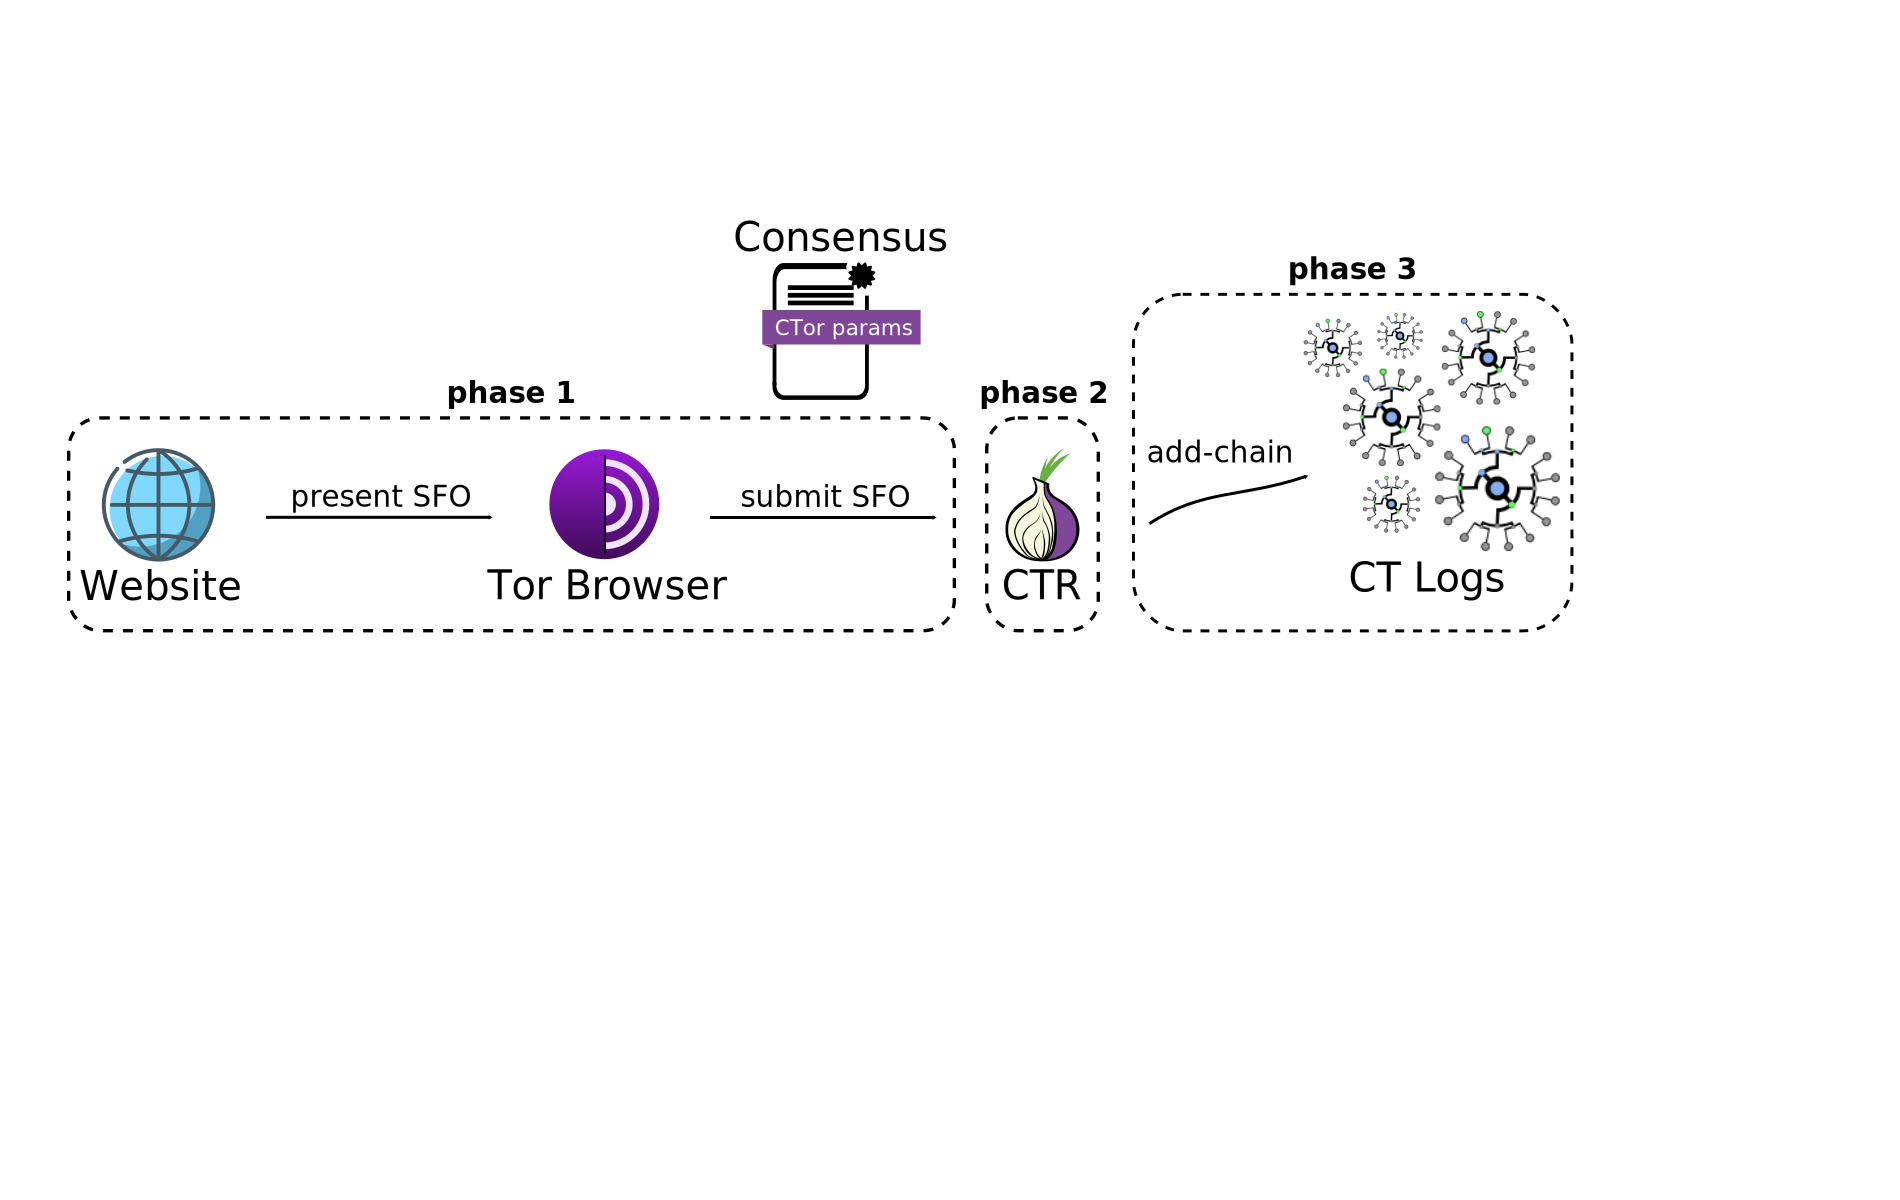
\includegraphics[width=0.85\textwidth]{img/design-ca}
	\caption{%
		The base design of CTor divided into three phases. A website presents an
		SFO to Tor Browser, and Tor Browser in turn with some probability
		submits the SFO to a random CTR (phase 1). A CTR stores the SFO a period
		of time (phase 2). The CTR adds the certificate in the SFO to a random
		independent CT log (phase 3).
	}
	\label{fig:design-ca}
\end{figure*}

\subsection{Tor Consensus} \label{sec:base:consensus}
Our proposal extends Tor's consensus document
so that it entails information regarding
	CTRs,
	recognized CT logs, and
	other necessary parameters that can be tuned.

\subsubsection{CTR Flag} \label{sec:base:consensus:ctr-flag}
The existing \texttt{known-flags} item determines the different flags that a 
given consensus document might contain.  We add another flag named \texttt{CTR},
which indicates that a Tor relay should support CT-auditing as described in
Sections~\ref{sec:base:phase2}--\ref{sec:base:phase3}.  A relay qualifies as a
CTR if it is flagged as \texttt{Stable} and not \texttt{Exit}.  As such, we
suggest using resources that are more abundant when compared to, e.g., exit
bandwidth.  A relay is assigned the \texttt{CTR} flag if a majority of directory
authorities voted for it.

TODO: elaborate 1-2 sentences why this ctr criteria and what it entails (?)

\subsubsection{Recognized CT Log} \label{sec:base:consensus:log}
CTRs only interact with CT logs that are recognized by the Tor consensus.  A log
is recognized if a majority of directory authorities voted for its inclusion by
proposing a \texttt{ct-log-info} entry that contains a log ID, a public key, and
a base URL~\cite{ct,ct/bis}. 
Following from our basic CTR design, there need not be any overlap between the
logs that the Tor consensus recognizes when compared to Tor Browser's CT policy.
There could be overlap, however.  The ideal scenario is that there are many
independent logs that accept certificate chains for most trust anchors.  We
discuss whether this is currently the case or not in Section~\ref{sec:todo}.  In
favor of brevity, details on how the Tor consensus captures whether two logs are
independent and which trust anchors they accept are omitted.

TODO: wrap-up here instead without any forward ref

\subsubsection{Other Parameters} \label{sec:base:consensus:params}
Directory authorities influence the way in which Tor Browser and CTRs behave by
voting on other necessary parameters.  For example, the likelihood that
an SFO is submitted to a CTR is a security parameter that is determined by the
value of \texttt{ct-submit-pr}.  Below, the value of an item is computed as the
median of all votes.
\begin{description}
	\item[ct-submit-pr:] A floating-point in $[0,1]$ that determines Tor
		Browser's submission probability.  For example, $0$ disables submissions
		while $0.10$ means that every 10$^{\mathsf{th}}$ SFO is sent to a
		random CTR on average.
	\item[ct-sfo-max-bytes:] A natural number that determines how many
		wire-bytes a normal SFO should not exceed.  As outlined in
		Section~\ref{sec:base:phase1}, excessively large SFOs are subject
		to stricter verification criteria.
	\item[ct-log-timeout:] A natural number that determines how long a CTR
		waits before concluding that a CT log is unresponsive, e.g., 10~seconds.
		As outlined in Section~\ref{sec:base:phase3}, timeouts trigger implicit
		resubmissions.
	\item[ct-delay-dist:] A distribution that determines how long a CTR should
		wait at minimum before auditing a submitted SFO\@.  As outlined in
		Section~\ref{sec:base:phase2}, random noise is added, e.g., on the order of minutes to an hour.
	\item[ct-backoff-dist:]
		A distribution that determines how long a CTR should wait between two
		auditing instances, e.g., a few minutes on average.  As outlined in
		Section~\ref{sec:base:phase3}, CTRs audit pending SFOs in batches at
		random time intervals to spread out log overhead.
\end{description}

The parameter \texttt{ct-delay-dist} is fulfilling two goals by adding
a randomized delay to the time a CTR should wait before auditing a
submitted SFO\@. For the base design, if a client visits a website and
then an associated SFO is submitted to a CT log shortly thereafter,
this could leak information about client behavior. As an extreme
example, if a known client is unique in visiting a specific collection
of websites together within a short period, seeing associated SFOs for
websites in that collection could indicate to a CT log the behavior of
that client. The randomness in whether a client submits and the
randomness of \texttt{ct-backoff-dist} might help complicate such
leakage. But both of these are primarily for overhead and perfomance,
and the latter is only on the order of minutes. \texttt{ct-delay-dist}
provides a guarantee of behavior obfuscation. 

For the base design, as well as the auditor extension of
Section~\ref{sec:auditor} and log extension of Section~\ref{sec:log},
\texttt{ct-delay-dist} provides some protection against flooding
attacks. Since the available memory of a CTR is known, by flooding
that CTR with enough SFOs before MMD of a mis-issued SCT, the
adversary could flush the desired SFO from the CTR and it would thus
never be audited.  Also for the extensions, if SFOs were audited as
soon as MMD was reached, then an adversary could be more efficient
about knowing when to flood the CTR\@. This could possibly even make
flooding of all CTRs in the network feasible. Even if auditing order
were randomized among all SFOs within an exact interval after MMD (a
timed mix), when to flood a CTR would be predictable. Adding a
randomized delay makes something akin to a stop-and-go mix, except
that the delay time is set by the CTR not the client, which is fine
since this aspect is not to protect client identity but to resist DoS
of SFO audit. Consult the literature~\cite{trickle02} for a description
of mix types.

If the storage strategy against flooding favored preserving SFOs
already at the CTR by dropping inbound SFOs or those farthest from
auditing, the adversary could optimize flooding to just before or
shortly after the mis-issued SFO is sent. If the storage strategy
against flooding favored not blocking incoming SFOs by dropping those
closest to being audited, then the adversary could optimize flooding
to after the mis-issued SFO is sent and as close to MMD as will make
flushing of it likely. To prevent useful optimization of flooding,
when storage capacity at a CTR is exceeded we thus select randomly
from among the pool of received SFOs regardless of time till audit.
And \texttt{ct-delay-dist} similarly complicates any attempted
optimization of when to flood a CTR, thus increasing average cost
of any such DoS attack for the adversary.


\subsection{Phase~1---Tor Browser} \label{sec:base:phase1}
The first phase covers Tor Browser and how an SFO is validated in the TLS
handshake.  We rely on Tor Browser's trust store to check certificate chains, an
assumed SCT-centric CT policy similar to Chrome~\cite{chrome-policy} and
Safari~\cite{safari-policy} to avoid breakage, and \texttt{ct-max-sfo-bytes} as
well as \texttt{ct-submit-pr} to determine whether and how there should be any
follow-up auditing that goes beyond SCT signature verification.  Given an
incoming SFO $s$:

\begin{enumerate}
	\item Raise a certificate error and stop if the certificate chain of $s$
		is not rooted in Tor Browser's trust store.
	\item Raise a certificate transparency error and stop if the SCTs of $s$
		fail Tor Browser's SCT-centric CT policy.
	\item Accept $s$ and conduct the remaining steps in the background if
		$\mathsf{len}(s) \le \texttt{ct-max-sfo-bytes}$, otherwise complete
		all steps and then accept~$s$ as valid.
	\item Flip a biased coin based on \texttt{ct-submit-pr} and stop if the
		outcome indicates no further auditing.
	\item Submit $s$ to a sampled CTR's SFO-endpoint on a pre-built CT-circuit.
		The circuit used for submission is closed immediately after use without
		waiting for any acknowledgment.
\end{enumerate}

In other words, an SFO is accepted as valid if the end-entity certificate is
rooted in a trust anchor \emph{and} it has enough SCTs as dictated by an
SCT-centric CT policy.  The decision and possible submission of an SFO to a
random CTR should never block the TLS handshake under normal circumstances,
whereas \emph{excessively large} SFOs do due to high security risks.  See
Section~\ref{sec:analysis:pr:phase1}, which also motivates why it is paramount
that submission circuits are pre-built and closed as soon as possible.

%
% - close circuit asap to make it harder for an attacker to figure out which
% CTR received a submission (should it have access to a zero-day takeover).
% - clearly a submission circuit cannot be reused across tabs, but not doing
% so within tabs may (i) reduce the chance that the receiving CTR knows exactly
% which website was visited, and (ii) make sense because with small submission
% pr (<=1/10) it should be common to submit at most once per tab anyway.
%

\subsection{Phase 2---Storage} \label{sec:base:phase2}
We suggest that CTRs accept SFO submissions on an HTTP endpoint.\footnote{%
	Tor's HTTP DirServer codebase can be reused as extension point to interact
	with the tor daemon, i.e., add another listener.
} For example, Nordberg~\emph{et~al.} defined an SCT feedback interface that can
be reused if an array-length of one is enforced by the CTR~\cite{nordberg}.
With regards to some CT circuit, process an incoming SFO $s$ as follows:
\begin{enumerate}
	\item\label{enm:storage:close} Close the current circuit to enforce one-time
		usage.
	\item\label{enm:storage:unrecognized} Stop if no CT log in the Tor consensus
		accepts the trust anchor of the underlying certificate chain in $s$.
	\item\label{enm:storage:cached}
		Stop if $s$ is cached or pending to be audited already.
	\item\label{enm:storage:fix-log} Sample an independent CT log $l$ that
		issued no SCT in $s$.  If there are no independent CT logs listed in the
		Tor consensus, sample a dependent CT log instead.
	\item\label{enm:storage:audit-after} Compute an \texttt{audit\_after}
		timestamp $\textrm{t} \gets \mathsf{now()} +
			\mathsf{random}(\texttt{ct-delay-dist})$.
		The former returns the current time and the latter a random delay.
	\item\label{enm:storage:store} Add $(l,t,s)$ to a buffer of pending SFOs.
\end{enumerate}

An SFO that
	(i) cannot be audited with regards to a CT log that the Tor consensus
		recognizes,
	(ii) is already audited as indicated by a \emph{cache}, or
	(iii) is pending to be audited in a \emph{buffer} of pending SFOs,
is discarded.  In contrast, a new SFO is stored in the CTR's buffer
alongside an \texttt{audit\_after} timestamp and a sampled CT log.  The
\texttt{audit\_after} timestamp specifies the earliest point in time that an SFO
will be audited in phase~3, which adds random noise that obfuscate real-time
browsing patterns in the Tor network.  Auditing is also fixed at this stage with
regards to some CT log, notably including resubmissions.  If memory becomes a
scarce resource, e.g., due to flooding, delete pending SFOs at
random~\cite{nordberg}.

\subsection{Phase 3---Auditing} \label{sec:base:phase3}
Each CTR maintains a single Tor circuit that is used to interact with CT logs
that have \texttt{ct-log-info} items.  At random time intervals, separate
auditing instances are initiated for each of these logs.  Given a known CT log~%
$l$:
\begin{enumerate}
	\item\label{enm:auditing:backoff} Sample a delay $d \gets
		\mathsf{random}(\texttt{ct-backoff-dist})$.
	\item\label{enm:auditing:sleep} Schedule a timer, waiting until $d$
		time units elapsed.
	\item\label{enm:auditing:loop} For each pending buffer entry $(l',s,t)$:
		\begin{enumerate}
			\item\label{enm:auditing:log-check} Continue the loop if $l\ne l'$.
			\item\label{enm:auditing:timestamp-check} Continue the loop if
				$t > \mathsf{now}()$.
			\item\label{enm:auditing:add-chain} Use \texttt{ct-log-timeout} to
				set a timer and add the certificate chain in $s$ to $l$ using
				the public \texttt{add-chain}~\cite{ct} or
				\texttt{submit-entry}~\cite{ct/bis} endpoints.
				\begin{itemize}
					\item\label{enm:auditing:add-chain:success} On valid
						SCT: cache the SFO, then discard it from the buffer of
						pending SFOs.
					\item\label{enm:auditing:add-chain:fail} On any other
						outcome: break the loop.
				\end{itemize}
		\end{enumerate}
	\item\label{enm:auditing:restart} Go back to
		step~\ref{enm:auditing:backoff}.
\end{enumerate}

As shown above we take an unusual approach towards auditing SFOs.  Rather than
following up on an SFO's inclusion status, the underlying certificate chain is
\emph{added} to a random CT log
	(see Section~\ref{sec:base:phase2}, step~\ref{enm:storage:fix-log}).
As such, the end-entity certificate is disclosed to public scrutiny and the
issuing CA will be held accountable if the log in question is honest.  A request
to add the certificate chain is considered successful if a valid SCT is returned
within a timely manner.  On any other outcome, such as invalid SCT signature or
timeout, the SFO remains in the buffer as the loop breaks and the CTR backs-off
in hope that the log becomes available again after wake-up.

Note that the auditing instances of different CT logs are separated.  This
assures that the unavailability of one CT log does not halt auditing of
unrelated buffer entries.

%If there is no independent log listed in the Tor consensus, it is
%still valuable to resubmit to a dependent log:
%	it might be the case that the attacker has access to a log's signing key,
%	but not the log's actual infrastructure.
%In other words, a mis-issued certificate would make it into the public domain
%in such a scenario if we resubmit it rather than discarding it due to lack of
%an independent log.

%%% Local Variables: 
%%% mode: latex 
%%% TeX-master: "../main"
%%% End:          
